\documentclass[
  12pt,
  openany,
  oneside,
  a4paper,
  brazil
]{abntex2}

\usepackage[T1]{fontenc}
\usepackage[utf8]{inputenc}
\usepackage[brazil]{babel}
\usepackage{array}
\usepackage{booktabs}
\usepackage{graphicx}
\usepackage{longtable}
\usepackage{tabularx}
\usepackage{hyperref}
\usepackage{enumitem}
\usepackage{float}
\usepackage{tikz}
\usepackage{xcolor}
\usetikzlibrary{positioning,arrows.meta,shapes.geometric,shapes.multipart}
\graphicspath{{plantuml/exportados/}{docs/plantuml/exportados/}}

\hypersetup{
  colorlinks=true,
  linkcolor=black,
  urlcolor=blue
}

\setlist[itemize]{noitemsep, topsep=4pt}
\setlength{\parindent}{1.25cm}
\setlength{\parskip}{0.2cm}
\setlrmarginsandblock{3cm}{2cm}{*}
\setulmarginsandblock{3cm}{2cm}{*}
\checkandfixthelayout

\newcommand{\ProjetoNome}{Site de Assinatura do EvoPG}
\newcommand{\AutorNome}{Matheus Veiga Bacetic Joaquim\\RA: 10425638\\[0.4cm]Beatriz Aparecida de Mello Barbosa\\RA: 10354067}
\newcommand{\InstituicaoNome}{Universidade Presbiteriana Mackenzie}
\newcommand{\CursoNome}{Ci\^encia da Computa\c{c}\~ao}
\newcommand{\DisciplinaNome}{Laborat\'orio de Engenharia de Software}
\newcommand{\ProfessorNome}{Gustavo Scalabrini Sampaio}
\newcommand{\AnoDocumento}{2026}

\titulo{Documenta\c{c}\~ao do Projeto \ProjetoNome}
\autor{\AutorNome}
\local{}
\data{\AnoDocumento}
\instituicao{
  \InstituicaoNome\\
  \CursoNome
}
\tipotrabalho{Documenta\c{c}\~ao acad\^emica de projeto}
\preambulo{Documento desenvolvido para a disciplina \DisciplinaNome, sob orienta\c{c}\~ao do professor \ProfessorNome.}

\begin{document}
\imprimircapa
\imprimirfolhaderosto*

\pdfbookmark[0]{\contentsname}{toc}
\tableofcontents
\clearpage

\chapter{Introdu\c{c}\~ao}
O projeto \ProjetoNome{} consiste no desenvolvimento de um site web responsivo voltado \`a apresenta\c{c}\~ao comercial do sistema EvoPG, \`a contrata\c{c}\~ao do plano e ao gerenciamento inicial da conta do cliente. Diferentemente da plataforma principal de gest\~ao, este projeto tem como foco a camada de entrada do produto, isto \'e, o ambiente em que o visitante conhece a solu\c{c}\~ao, realiza a assinatura e acessa funcionalidades relacionadas \`a sua conta.

At\'e o momento, o projeto encontra-se em fase de defini\c{c}\~ao, prototipa\c{c}\~ao e estrutura\c{c}\~ao arquitetural. J\'a existe material inicial de interface institucional e refer\^encias t\'ecnicas para integra\c{c}\~oes, por\'em o site de assinatura propriamente dito ainda ser\'a desenvolvido nas pr\'oximas etapas. Assim, esta documenta\c{c}\~ao descreve o produto pretendido, os requisitos previstos, os prot\'otipos iniciais, a modelagem leve e a arquitetura planejada para sua implementa\c{c}\~ao.

\chapter{Defini\c{c}\~ao da demanda}

\section{Problema ou oportunidade percebida}
Mesmo quando uma plataforma de gest\~ao oferece recursos relevantes, sua ado\c{c}\~ao pode ser comprometida se n\~ao houver um site claro para apresentar a proposta do produto, explicar planos, converter visitantes em assinantes e permitir o gerenciamento da conta do cliente. Sem essa camada, o processo comercial e de onboarding tende a ficar fragmentado, pouco profissional e dependente de abordagens manuais.

Nesse contexto, surge a oportunidade de desenvolver um site de assinatura dedicado ao EvoPG, capaz de funcionar como ponte entre o interesse inicial do cliente e o acesso efetivo ao servi\c{c}o. Esse site deve apoiar a convers\~ao comercial, organizar o fluxo de assinatura e concentrar informa\c{c}\~oes b\'asicas de conta e integra\c{c}\~oes.

\section{Raz\~ao ou justificativa da demanda}
A demanda se justifica pela necessidade de:
\begin{itemize}
  \item apresentar o EvoPG de forma clara e profissional para novos clientes;
  \item permitir a assinatura do servi\c{c}o em fluxo digital centralizado;
  \item reduzir depend\^encia de processos manuais para cobran\c{c}a e ativa\c{c}\~ao de conta;
  \item oferecer ao cliente um espa\c{c}o inicial para login, perfil, dados cadastrais e integra\c{c}\~oes;
  \item estruturar uma experi\^encia de entrada coerente com o modelo SaaS do produto.
\end{itemize}

\section{Descri\c{c}\~ao sucinta do produto de software}
O \ProjetoNome{} \'e um site web de assinatura que pretende combinar uma camada comercial de aquisi\c{c}\~ao de clientes, por meio da landing page, com uma camada transacional de cadastro e acesso. Em sua vers\~ao planejada, o sistema dever\'a permitir:
\begin{itemize}
  \item apresenta\c{c}\~ao do EvoPG e capta\c{c}\~ao de potenciais assinantes;
  \item contrata\c{c}\~ao do plano por meio de um site de assinatura, que ainda ser\'a desenvolvido;
  \item exibi\c{c}\~ao dos termos de uso antes do redirecionamento ao pagamento;
  \item cria\c{c}\~ao autom\'atica da conta ap\'os pagamento aprovado;
  \item envio de e-mail para defini\c{c}\~ao ou redefini\c{c}\~ao da senha inicial;
  \item autentica\c{c}\~ao por senha, link m\'agico e recupera\c{c}\~ao de senha;
  \item gerenciamento do perfil e da conta do usu\'ario;
  \item preenchimento da ficha fiscal de empresa ou pessoa f\'isica;
  \item acompanhamento do status da assinatura e bloqueio por inadimpl\^encia;
  \item integra\c{c}\~ao com Mercado Pago para opera\c{c}\~oes de cobran\c{c}a;
  \item envio de mensagens para suporte pelo pr\'oprio site.
\end{itemize}

\section{Clientes, usu\'arios e demais envolvidos}
\textbf{Clientes do produto:} micro e pequenas empresas, empreendedores individuais e gestores interessados em contratar o EvoPG.

\textbf{Usu\'arios diretos:} visitantes do site, assinantes do EvoPG, administradores da conta e equipe comercial ou de suporte.

\textbf{Envolvidos e impactados:}
\begin{itemize}
  \item equipe de desenvolvimento e manuten\c{c}\~ao do site;
  \item suporte ao cliente;
  \item provedores externos integrados, como Supabase, Stripe, Mercado Pago e servi\c{c}o de e-mail;
  \item equipe respons\'avel pela plataforma principal do EvoPG;
  \item usu\'arios finais que dependem de estabilidade, seguran\c{c}a e clareza das informa\c{c}\~oes exibidas.
\end{itemize}

\section{Principais etapas para construir o produto}
De forma geral, a constru\c{c}\~ao do produto envolve:
\begin{enumerate}
  \item levantamento da demanda e defini\c{c}\~ao do escopo inicial;
  \item modelagem dos processos principais e dos dados essenciais;
  \item prototipa\c{c}\~ao das interfaces principais;
  \item implementa\c{c}\~ao da landing page e do site de assinatura;
  \item implementa\c{c}\~ao do backend serverless e banco de dados;
  \item integra\c{c}\~ao com autentica\c{c}\~ao, cobran\c{c}a, pagamento e gerenciamento de conta;
  \item valida\c{c}\~ao funcional, ajustes de usabilidade e revis\~ao da experi\^encia;
  \item implanta\c{c}\~ao em ambiente de produ\c{c}\~ao e evolu\c{c}\~ao cont\'inua.
\end{enumerate}

\section{Principais crit\'erios de qualidade}
Os principais crit\'erios de qualidade definidos para o \ProjetoNome{} s\~ao:
\begin{itemize}
  \item \textbf{Usabilidade:} telas objetivas, linguagem clara e navega\c{c}\~ao simples;
  \item \textbf{Confiabilidade:} tratamento de falhas, consist\^encia dos dados e regras de neg\'ocio para acesso por assinatura;
  \item \textbf{Seguran\c{c}a:} autentica\c{c}\~ao, prote\c{c}\~ao de dados, valida\c{c}\~ao de entradas e integra\c{c}\~oes seguras;
  \item \textbf{Desempenho:} carregamento r\'apido das p\'aginas e respostas adequadas nas integra\c{c}\~oes;
  \item \textbf{Escalabilidade:} capacidade de ampliar o n\'umero de clientes e integra\c{c}\~oes sem reescrever toda a solu\c{c}\~ao;
  \item \textbf{Manutenibilidade:} c\'odigo organizado em arquivos separados por responsabilidade;
  \item \textbf{Disponibilidade:} acesso web cont\'inuo, com depend\^encia controlada de servi\c{c}os externos.
\end{itemize}

\chapter{Requisitos do produto}

\section{Tabela de requisitos}
\renewcommand{\arraystretch}{1.2}
\begin{longtable}{>{\raggedright\arraybackslash}p{1.8cm} >{\raggedright\arraybackslash}p{1.8cm} >{\raggedright\arraybackslash}p{2cm} >{\raggedright\arraybackslash}p{8.8cm}}
\toprule
\textbf{ID} & \textbf{Tipo} & \textbf{Prioridade} & \textbf{Descri\c{c}\~ao} \\
\midrule
\endfirsthead
\toprule
\textbf{ID} & \textbf{Tipo} & \textbf{Prioridade} & \textbf{Descri\c{c}\~ao} \\
\midrule
\endhead
RF01 & RF & Alta & O sistema deve apresentar uma landing page com descri\c{c}\~ao do EvoPG, benef\'icios, planos e chamada para assinatura. \\
RF02 & RF & Alta & O sistema deve possuir um site de assinatura para iniciar a contrata\c{c}\~ao do plano. \\
RF03 & RF & Alta & O sistema deve exibir os termos de uso e exigir aceite antes do redirecionamento ao pagamento. \\
RF04 & RF & Alta & O sistema deve permitir autentica\c{c}\~ao por e-mail e senha. \\
RF05 & RF & Alta & O sistema deve permitir autentica\c{c}\~ao por link m\'agico enviado por e-mail. \\
RF06 & RF & Alta & O sistema deve permitir recupera\c{c}\~ao e redefini\c{c}\~ao de senha. \\
RF07 & RF & Alta & O sistema deve exibir uma \'area de perfil com identifica\c{c}\~ao do usu\'ario autenticado e dados da conta. \\
RF08 & RF & Alta & O sistema deve permitir ao usu\'ario acessar uma \'area de gerenciamento da assinatura. \\
RF09 & RF & Alta & O sistema deve registrar e consultar o status de pagamento da assinatura quando o m\'odulo de assinatura estiver implantado. \\
RF10 & RF & Alta & O sistema deve bloquear o acesso quando a assinatura estiver em estado de inadimpl\^encia bloqueada. \\
RF11 & RF & Alta & O sistema deve permitir cadastrar ficha fiscal para pessoa jur\'idica, incluindo CNPJ, IE, IM e regime tribut\'ario. \\
RF12 & RF & Alta & O sistema deve permitir cadastrar ficha fiscal para pessoa f\'isica, incluindo CPF. \\
RF13 & RF & Alta & O sistema deve permitir editar e salvar os dados fiscais do cadastro. \\
RF14 & RF & M\'edia & O sistema deve permitir conectar uma conta do Mercado Pago via OAuth. \\
RF15 & RF & M\'edia & O sistema deve permitir consultar o status da integra\c{c}\~ao com Mercado Pago. \\
RF16 & RF & M\'edia & O sistema deve permitir desconectar a conta integrada do Mercado Pago. \\
RF17 & RF & M\'edia & O sistema deve disponibilizar canal de contato com o suporte diretamente no site. \\
RF18 & RF & M\'edia & O sistema deve registrar eventos de integra\c{c}\~ao para auditoria e acompanhamento. \\
RF19 & RF & M\'edia & O sistema deve manter informa\c{c}\~oes da assinatura associadas \`a empresa cadastrada. \\
RF20 & RF & Baixa & O site deve permitir expans\~ao futura para novas integra\c{c}\~oes relacionadas \`a conta do cliente. \\
RF21 & RF & Alta & O sistema deve redirecionar o usu\'ario ao Stripe para que ele informe os dados iniciais e realize o pagamento. \\
RF22 & RF & Alta & O sistema deve criar automaticamente a conta do cliente ap\'os a confirma\c{c}\~ao do pagamento aprovado. \\
RF23 & RF & Alta & O sistema deve enviar um e-mail para defini\c{c}\~ao ou redefini\c{c}\~ao da senha inicial ap\'os a cria\c{c}\~ao da conta. \\
RNF01 & RNF & Alta & O sistema deve operar em ambiente web responsivo, acess\'ivel em desktop e dispositivos m\'oveis. \\
RNF02 & RNF & Alta & O sistema deve validar os dados informados antes do envio para os servi\c{c}os externos. \\
RNF03 & RNF & Alta & O sistema deve proteger autentica\c{c}\~ao e integra\c{c}\~oes por meio de chaves, tokens e verifica\c{c}\~oes seguras. \\
RNF04 & RNF & Alta & O sistema deve preservar a consist\^encia dos dados de pagamento e do status de acesso. \\
RNF05 & RNF & Alta & O sistema deve permitir manuten\c{c}\~ao modular, separando interface, scripts e fun\c{c}\~oes backend. \\
RNF06 & RNF & M\'edia & O sistema deve fornecer mensagens claras de erro e sucesso ao usu\'ario. \\
RNF07 & RNF & M\'edia & O sistema deve ter tempo de resposta adequado para opera\c{c}\~oes principais de autentica\c{c}\~ao e checkout. \\
RNF08 & RNF & M\'edia & O sistema deve suportar evolu\c{c}\~ao incremental de integra\c{c}\~oes sem altera\c{c}\~ao radical da arquitetura. \\
\bottomrule
\end{longtable}

\section{Backlog do produto}
\begin{longtable}{>{\raggedright\arraybackslash}p{1.8cm} >{\raggedright\arraybackslash}p{7.2cm} >{\raggedright\arraybackslash}p{2.2cm} >{\raggedright\arraybackslash}p{3.3cm}}
\toprule
\textbf{Item} & \textbf{Hist\'oria ou entrega} & \textbf{Prioridade} & \textbf{Situa\c{c}\~ao} \\
\midrule
\endfirsthead
\toprule
\textbf{Item} & \textbf{Hist\'oria ou entrega} & \textbf{Prioridade} & \textbf{Situa\c{c}\~ao} \\
\midrule
\endhead
B01 & Como visitante, quero entender a proposta do EvoPG para avaliar a assinatura. & Alta & Planejado \\
B02 & Como cliente, quero contratar o plano online para obter acesso ao servi\c{c}o. & Alta & Planejado \\
B03 & Como visitante, quero aceitar os termos de uso antes de prosseguir com a assinatura. & Alta & Planejado \\
B04 & Como cliente, quero receber um e-mail para definir minha senha inicial ap\'os o pagamento. & Alta & Planejado \\
B05 & Como cliente, quero preencher minha ficha fiscal para concluir meu cadastro. & Alta & Planejado \\
B06 & Como gestor do sistema, quero controlar inadimpl\^encia para restringir acesso quando necess\'ario. & Alta & Planejado \\
B07 & Como cliente, quero gerenciar minha assinatura para manter meu plano ativo. & Alta & Planejado \\
B08 & Como usu\'ario, quero entrar com senha ou link m\'agico para acessar minha conta. & Alta & Planejado \\
B09 & Como cliente, quero conectar Mercado Pago para usar cobran\c{c}a integrada. & M\'edia & Planejado \\
B10 & Como administrador, quero registrar eventos de integra\c{c}\~ao para fins de rastreabilidade. & M\'edia & Planejado \\
B11 & Como visitante, quero falar com o suporte sem sair do site. & M\'edia & Planejado \\
B12 & Como cliente, quero acompanhar o status da minha assinatura e da minha conta. & M\'edia & Planejado \\
B13 & Como cliente, quero acessar um ambiente inicial de conta com meus dados cadastrais. & M\'edia & Planejado \\
B14 & Como administrador, quero expandir o site para novas integra\c{c}\~oes futuras. & Baixa & Planejado \\
\bottomrule
\end{longtable}

\chapter{Wireframes}
Os wireframes abaixo representam prot\'otipos de baixa fidelidade das telas principais identificadas no escopo atual do projeto. O objetivo n\~ao \'e reproduzir a interface visual final, mas evidenciar estrutura, hierarquia de informa\c{c}\~ao e fluxo de navega\c{c}\~ao.

\section{Tela 1: Landing page}
\begin{figure}[H]
\centering
\begin{tikzpicture}[x=1cm,y=1cm]
  \draw (0,0) rectangle (14,9);
  \draw (0.4,8.2) rectangle (13.6,8.7);
  \node[anchor=west] at (0.7,8.45) {Logo};
  \node[anchor=east] at (13.2,8.45) {Login / Cadastre-se};
  \draw (0.8,5.2) rectangle (7.2,7.8);
  \node at (4,7.2) {Headline do produto};
  \node at (4,6.5) {Subt\'itulo com proposta de valor};
  \draw (2.3,5.6) rectangle (5.7,6.0);
  \node at (4,5.8) {CTA de assinatura};
  \draw (8.1,5.1) rectangle (13.0,7.8);
  \node at (10.55,6.45) {V\'ideo / demonstra\c{c}\~ao};
  \draw (0.8,2.8) rectangle (4.9,4.5);
  \draw (5.1,2.8) rectangle (9.2,4.5);
  \draw (9.4,2.8) rectangle (13.0,4.5);
  \node at (2.85,3.65) {Card\\Financeiro};
  \node at (7.15,3.65) {Card\\Relat\'orios};
  \node at (11.2,3.65) {Card\\Opera\c{c}\~ao};
  \draw (0.8,0.8) rectangle (13.0,2.1);
  \node at (6.9,1.45) {Planos, integra\c{c}\~oes, FAQ e suporte};
\end{tikzpicture}
\caption{Prot\'otipo de baixa fidelidade da landing page}
\end{figure}

\section{Tela 2: Acesso e perfil}
\begin{figure}[H]
\centering
\begin{tikzpicture}[x=1cm,y=1cm]
  \draw (0,0) rectangle (14,9);
  \draw (0.6,8.1) rectangle (3.0,8.6);
  \node at (1.8,8.35) {Voltar};
  \draw (0.8,0.8) rectangle (13.2,7.7);
  \draw (1.2,6.4) rectangle (12.8,7.2);
  \node at (7,6.8) {Nome / E-mail / ID do usu\'ario};
  \draw (1.2,5.4) rectangle (4.0,6.0);
  \node at (2.6,5.7) {Assinatura};
  \draw (4.3,5.4) rectangle (7.1,6.0);
  \node at (5.7,5.7) {Empresa};
  \draw (7.4,5.4) rectangle (10.2,6.0);
  \node at (8.8,5.7) {Integra\c{c}\~oes};
  \draw (10.5,5.4) rectangle (12.8,6.0);
  \node at (11.65,5.7) {Senha};
  \draw (1.2,2.6) rectangle (8.5,4.9);
  \node at (4.85,4.4) {Ficha fiscal};
  \node at (4.85,3.8) {CNPJ ou CPF};
  \node at (4.85,3.2) {IE / IM / Regime tribut\'ario};
  \draw (9.0,2.6) rectangle (12.8,4.9);
  \node at (10.9,4.2) {Mercado Pago};
  \node at (10.9,3.6) {Status};
  \node at (10.9,3.0) {Conectar / Atualizar / Desconectar};
  \draw (4.6,1.2) rectangle (9.4,2.0);
  \node at (7,1.6) {Bot\~ao Ir para a plataforma};
\end{tikzpicture}
\caption{Prot\'otipo de baixa fidelidade da \'area de perfil}
\end{figure}

\section{Tela 3: Site de assinatura}
\begin{figure}[H]
\centering
\begin{tikzpicture}[x=1cm,y=1cm]
  \draw (0,0) rectangle (14,8);
  \draw (1.0,5.7) rectangle (6.1,7.0);
  \node at (3.55,6.35) {Sele\c{c}\~ao do plano};
  \draw (7.1,5.7) rectangle (13.0,7.0);
  \node at (10.05,6.35) {Resumo da assinatura};
  \draw (1.0,3.5) rectangle (13.0,5.0);
  \node at (7,4.25) {Termos de uso e aceite LGPD};
  \draw (1.0,1.4) rectangle (6.1,2.8);
  \node at (3.55,2.1) {Aceitar e continuar};
  \draw (7.1,1.4) rectangle (13.0,2.8);
  \node at (10.05,2.1) {Redirecionar ao Stripe};
\end{tikzpicture}
\caption{Prot\'otipo de baixa fidelidade do site de assinatura}
\end{figure}

\chapter{Modelagem leve do sistema}
A modelagem leve do sistema foi organizada para representar, de forma objetiva, os principais atores, intera\c{c}\~oes, classes de dom\'inio e casos de uso do site de assinatura. O objetivo desta se\c{c}\~ao \'e evidenciar o comportamento essencial do sistema sem recorrer a uma modelagem excessivamente detalhada, mantendo foco no fluxo de contrata\c{c}\~ao, primeiro acesso e gerenciamento da conta.

\section{Vis\~ao geral dos atores}
Os principais atores do sistema s\~ao:
\begin{itemize}
  \item \textbf{Visitante:} navega pela landing page, consulta informa\c{c}\~oes e poder\'a iniciar a assinatura;
  \item \textbf{Cliente/usu\'ario autenticado:} acessa o perfil, mant\'em dados cadastrais e gerencia sua conta;
  \item \textbf{Administrador do servi\c{c}o:} acompanha assinaturas, integra\c{c}\~oes e suporte;
  \item \textbf{Servi\c{c}os externos:} Stripe, Mercado Pago, Supabase e servi\c{c}o de envio de e-mail.
\end{itemize}

\section{Diagrama de casos de uso}
\begin{figure}[H]
\centering
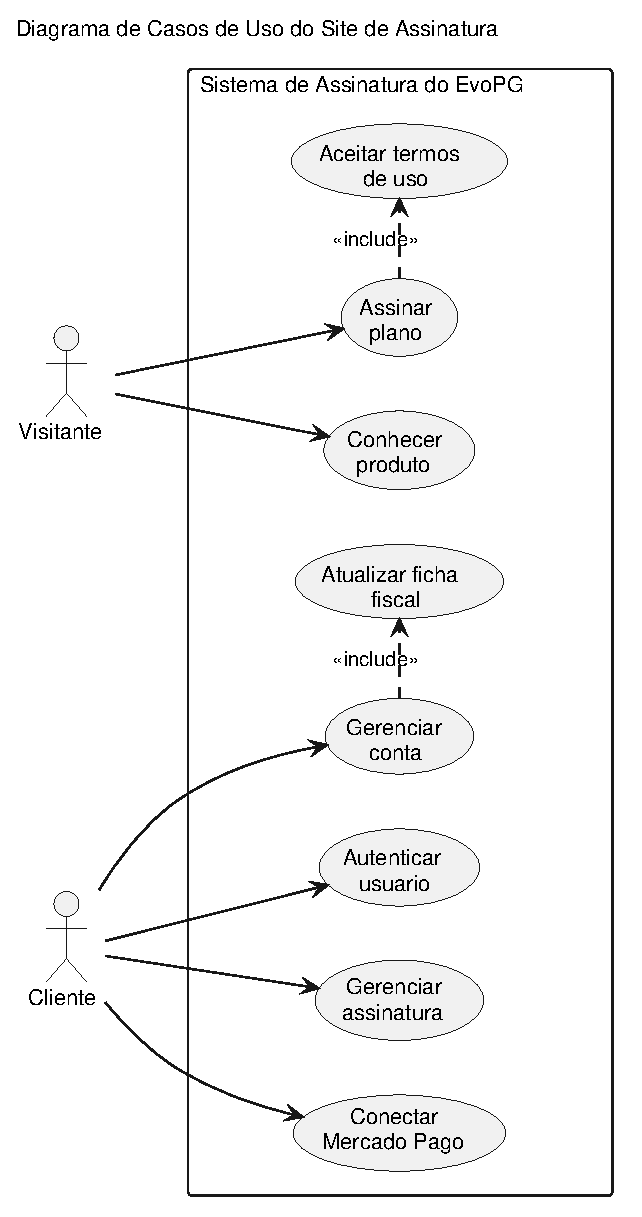
\includegraphics[width=0.9\textwidth,height=0.72\textheight,keepaspectratio]{casos_uso_assinatura}
\caption{Diagrama de casos de uso do site de assinatura}
\end{figure}
O diagrama evidencia que o caso de uso \textit{Assinar plano} depende da aceita\c{c}\~ao dos termos de uso e que os casos de primeiro acesso e autentica\c{c}\~ao ficam concentrados na jornada posterior \`a aprova\c{c}\~ao do pagamento.

\section{Casos de uso principais}
\begin{longtable}{>{\raggedright\arraybackslash}p{3.5cm} >{\raggedright\arraybackslash}p{10cm}}
\toprule
\textbf{Caso de uso} & \textbf{Descri\c{c}\~ao} \\
\midrule
Conhecer o produto & O visitante acessar\'a a landing page para entender a proposta do EvoPG, seus benef\'icios e planos. \\
Assinar plano & O visitante clicar\'a em assinar e iniciar\'a o fluxo de contrata\c{c}\~ao. \\
Aceitar termos de uso & O visitante dever\'a aceitar os termos de uso antes de prosseguir para o pagamento. \\
Redefinir senha inicial & O cliente receber\'a um e-mail ap\'os o pagamento aprovado para criar sua senha de acesso. \\
Autenticar usu\'ario & O cliente acessar\'a o sistema com a senha definida ou por meios alternativos previstos. \\
Gerenciar conta & O usu\'ario consultar\'a seus dados cadastrais, o status da assinatura e os recursos dispon\'iveis na conta. \\
Cadastrar ficha fiscal & O cliente salvar\'a dados de PJ ou PF necess\'arios ao contexto do produto. \\
Gerenciar assinatura & O usu\'ario acessar\'a a \'area relacionada ao pagamento recorrente. \\
Controlar acesso por cobran\c{c}a & O backend validar\'a se a empresa est\'a em dia, atrasada ou bloqueada. \\
Conectar Mercado Pago & O usu\'ario iniciar\'a o OAuth e autorizar\'a a integra\c{c}\~ao de pagamento. \\
Enviar mensagem ao suporte & O visitante ou cliente enviar\'a uma solicita\c{c}\~ao para atendimento. \\
\bottomrule
\end{longtable}

\section{Especifica\c{c}\~oes dos casos de uso principais}
As especifica\c{c}\~oes a seguir detalham os casos de uso considerados cr\'iticos para o fluxo de neg\'ocio do site de assinatura, isto \'e, a contrata\c{c}\~ao do plano, o primeiro acesso e a administra\c{c}\~ao da conta do cliente.

\subsection{UC01 -- Assinar plano}
\renewcommand{\arraystretch}{1.15}
\begin{longtable}{>{\raggedright\arraybackslash}p{3.3cm} >{\raggedright\arraybackslash}p{10cm}}
\toprule
\textbf{Campo} & \textbf{Descri\c{c}\~ao} \\
\midrule
\endfirsthead
\toprule
\textbf{Campo} & \textbf{Descri\c{c}\~ao} \\
\midrule
\endhead
Identificador & UC01 \\
Nome & Assinar plano \\
Objetivo & Permitir que um visitante inicie a contrata\c{c}\~ao do plano, aceite os termos, seja direcionado ao Stripe e tenha sua conta criada ap\'os pagamento aprovado. \\
Ator principal & Visitante \\
Interessados & Cliente, equipe comercial, sistema de pagamento e plataforma EvoPG. \\
Pr\'e-condi\c{c}\~oes & Landing page dispon\'ivel; plano publicado; integra\c{c}\~ao de pagamento configurada. \\
P\'os-condi\c{c}\~oes & Assinatura registrada; em caso de aprova\c{c}\~ao do pagamento, conta do cliente criada e fluxo de defini\c{c}\~ao de senha iniciado por e-mail. \\
Gatilho & O visitante clica no bot\~ao de assinatura. \\
Fluxo principal & 1. O visitante acessa a landing page. \newline 2. O sistema apresenta a proposta do produto e os planos. \newline 3. O visitante clica em assinar. \newline 4. O sistema exibe os termos de uso. \newline 5. O visitante aceita os termos. \newline 6. O sistema redireciona o visitante ao Stripe. \newline 7. No Stripe, o visitante informa os dados iniciais necess\'arios e realiza o pagamento. \newline 8. O Stripe processa a transa\c{c}\~ao. \newline 9. O sistema recebe a confirma\c{c}\~ao do pagamento aprovado. \newline 10. O sistema cria a conta do cliente. \newline 11. O sistema envia um e-mail para defini\c{c}\~ao ou redefini\c{c}\~ao de senha. \newline 12. O cliente fica apto a acessar a plataforma ap\'os definir sua senha. \\
Fluxos alternativos & A1. Se o visitante n\~ao aceitar os termos, o processo de assinatura n\~ao prossegue. \newline A2. Se o pagamento for recusado, a conta n\~ao \'e criada. \newline A3. Se houver falha na confirma\c{c}\~ao do pagamento, o sistema mant\'em a assinatura sem ativa\c{c}\~ao. \newline A4. Se o visitante abandonar o Stripe, o fluxo \'e encerrado sem conclus\~ao. \\
Regras de neg\'ocio & O aceite dos termos de uso e da pol\'itica de dados \'e obrigat\'orio; o pagamento aprovado \'e condi\c{c}\~ao para cria\c{c}\~ao da conta; o e-mail do comprador deve ser v\'alido para o envio da redefini\c{c}\~ao de senha. \\
\bottomrule
\end{longtable}

\subsection{UC02 -- Autenticar usu\'ario}
\begin{longtable}{>{\raggedright\arraybackslash}p{3.3cm} >{\raggedright\arraybackslash}p{10cm}}
\toprule
\textbf{Campo} & \textbf{Descri\c{c}\~ao} \\
\midrule
\endfirsthead
\toprule
\textbf{Campo} & \textbf{Descri\c{c}\~ao} \\
\midrule
\endhead
Identificador & UC02 \\
Nome & Autenticar usu\'ario \\
Objetivo & Permitir que o cliente acesse a \'area de conta e, posteriormente, a plataforma ap\'os definir sua senha inicial. \\
Ator principal & Cliente \\
Interessados & Cliente, equipe de suporte e plataforma EvoPG. \\
Pr\'e-condi\c{c}\~oes & Conta cadastrada no sistema; servi\c{c}o de autentica\c{c}\~ao dispon\'ivel; senha inicial j\'a definida, quando for o primeiro acesso. \\
P\'os-condi\c{c}\~oes & Sess\~ao autenticada iniciada; cliente redirecionado para a \'area de conta. \\
Gatilho & O cliente acessa a tela de login. \\
Fluxo principal & 1. O cliente acessa a p\'agina de autentica\c{c}\~ao. \newline 2. O sistema apresenta as op\c{c}\~oes de entrada. \newline 3. O cliente informa suas credenciais. \newline 4. O sistema valida a solicita\c{c}\~ao. \newline 5. O sistema autentica o usu\'ario. \newline 6. O sistema verifica se a conta pode acessar o servi\c{c}o. \newline 7. O cliente \'e direcionado para sua \'area de conta e pode seguir para a plataforma. \\
Fluxos alternativos & A1. Se as credenciais forem inv\'alidas, o sistema informa o erro. \newline A2. Se a conta estiver bloqueada por inadimpl\^encia, o sistema impede o acesso. \newline A3. Se o cliente ainda n\~ao tiver definido a senha, o sistema orienta o uso do link recebido por e-mail. \newline A4. Se o cliente esquecer a senha, o sistema oferece fluxo de recupera\c{c}\~ao. \\
Regras de neg\'ocio & O acesso depende da exist\^encia de uma conta v\'alida; a libera\c{c}\~ao pode ser limitada pela situa\c{c}\~ao da assinatura; no primeiro acesso a senha deve ser definida antes do login convencional. \\
\bottomrule
\end{longtable}

\subsection{UC03 -- Redefinir senha inicial}
\begin{longtable}{>{\raggedright\arraybackslash}p{3.3cm} >{\raggedright\arraybackslash}p{10cm}}
\toprule
\textbf{Campo} & \textbf{Descri\c{c}\~ao} \\
\midrule
\endfirsthead
\toprule
\textbf{Campo} & \textbf{Descri\c{c}\~ao} \\
\midrule
\endhead
Identificador & UC03 \\
Nome & Redefinir senha inicial \\
Objetivo & Permitir que o cliente defina sua senha de acesso ap\'os o pagamento aprovado e a cria\c{c}\~ao autom\'atica da conta. \\
Ator principal & Cliente \\
Interessados & Cliente, sistema de autentica\c{c}\~ao e plataforma EvoPG. \\
Pr\'e-condi\c{c}\~oes & Pagamento aprovado; conta criada; e-mail de redefini\c{c}\~ao enviado ao cliente. \\
P\'os-condi\c{c}\~oes & Senha inicial definida com sucesso e acesso liberado para autentica\c{c}\~ao normal. \\
Gatilho & O cliente acessa o link recebido por e-mail. \\
Fluxo principal & 1. O sistema envia o e-mail de redefini\c{c}\~ao. \newline 2. O cliente abre a mensagem recebida. \newline 3. O cliente clica no link de redefini\c{c}\~ao. \newline 4. O sistema apresenta a tela de defini\c{c}\~ao de senha. \newline 5. O cliente informa e confirma a nova senha. \newline 6. O sistema valida os dados informados. \newline 7. O sistema grava a senha. \newline 8. O cliente passa a poder acessar a plataforma autenticado. \\
Fluxos alternativos & A1. Se o link estiver expirado, o sistema solicita nova recupera\c{c}\~ao. \newline A2. Se as senhas n\~ao coincidirem, o sistema solicita corre\c{c}\~ao. \newline A3. Se a senha n\~ao atender \`as regras m\'inimas, o sistema rejeita a submiss\~ao. \\
Regras de neg\'ocio & O link deve ser de uso controlado; a senha deve obedecer aos crit\'erios m\'inimos definidos; somente contas efetivamente criadas podem concluir o processo. \\
\bottomrule
\end{longtable}

\subsection{UC04 -- Gerenciar conta}
\begin{longtable}{>{\raggedright\arraybackslash}p{3.3cm} >{\raggedright\arraybackslash}p{10cm}}
\toprule
\textbf{Campo} & \textbf{Descri\c{c}\~ao} \\
\midrule
\endfirsthead
\toprule
\textbf{Campo} & \textbf{Descri\c{c}\~ao} \\
\midrule
\endhead
Identificador & UC04 \\
Nome & Gerenciar conta \\
Objetivo & Permitir que o cliente visualize seus dados, acompanhe a assinatura e mantenha informa\c{c}\~oes cadastrais atualizadas. \\
Ator principal & Cliente \\
Interessados & Cliente, equipe de suporte e equipe administrativa do servi\c{c}o. \\
Pr\'e-condi\c{c}\~oes & Cliente autenticado. \\
P\'os-condi\c{c}\~oes & Dados da conta consultados ou atualizados com sucesso. \\
Gatilho & O cliente acessa a \'area de conta. \\
Fluxo principal & 1. O cliente entra na \'area autenticada. \newline 2. O sistema exibe dados de identifica\c{c}\~ao e status da conta. \newline 3. O cliente consulta as op\c{c}\~oes dispon\'iveis. \newline 4. O cliente atualiza informa\c{c}\~oes cadastrais ou fiscais. \newline 5. O sistema valida e salva as altera\c{c}\~oes. \newline 6. O sistema confirma a atualiza\c{c}\~ao. \\
Fluxos alternativos & A1. Se houver dados inv\'alidos, o sistema apresenta mensagem de corre\c{c}\~ao. \newline A2. Se houver falha de comunica\c{c}\~ao com o backend, a altera\c{c}\~ao n\~ao \'e persistida. \\
Regras de neg\'ocio & Campos fiscais devem obedecer ao formato exigido; apenas usu\'arios autenticados podem alterar dados da conta. \\
\bottomrule
\end{longtable}

\subsection{UC05 -- Conectar Mercado Pago}
\begin{longtable}{>{\raggedright\arraybackslash}p{3.3cm} >{\raggedright\arraybackslash}p{10cm}}
\toprule
\textbf{Campo} & \textbf{Descri\c{c}\~ao} \\
\midrule
\endfirsthead
\toprule
\textbf{Campo} & \textbf{Descri\c{c}\~ao} \\
\midrule
\endhead
Identificador & UC05 \\
Nome & Conectar Mercado Pago \\
Objetivo & Permitir que o cliente autorize a integra\c{c}\~ao da sua conta com o Mercado Pago. \\
Ator principal & Cliente \\
Interessados & Cliente, sistema EvoPG e servi\c{c}o Mercado Pago. \\
Pr\'e-condi\c{c}\~oes & Cliente autenticado; conta apta a configurar integra\c{c}\~oes. \\
P\'os-condi\c{c}\~oes & Integra\c{c}\~ao registrada como ativa ou mensagem de falha apresentada ao usu\'ario. \\
Gatilho & O cliente seleciona a op\c{c}\~ao de conectar Mercado Pago. \\
Fluxo principal & 1. O cliente acessa a se\c{c}\~ao de integra\c{c}\~oes. \newline 2. O sistema apresenta o status atual da integra\c{c}\~ao. \newline 3. O cliente solicita a conex\~ao. \newline 4. O sistema inicia o fluxo OAuth. \newline 5. O cliente autoriza o acesso no provedor externo. \newline 6. O sistema recebe a confirma\c{c}\~ao e registra a integra\c{c}\~ao. \newline 7. O sistema atualiza o status exibido na conta. \\
Fluxos alternativos & A1. Se o cliente cancelar a autoriza\c{c}\~ao, o sistema mant\'em a integra\c{c}\~ao inativa. \newline A2. Se ocorrer erro no provedor externo, o sistema informa a falha e permite nova tentativa. \\
Regras de neg\'ocio & Apenas clientes autenticados podem autorizar integra\c{c}\~oes; a integra\c{c}\~ao depende do retorno positivo do fluxo OAuth. \\
\bottomrule
\end{longtable}

\section{Diagrama de sequ\^encia principal}
\begin{figure}[H]
\centering
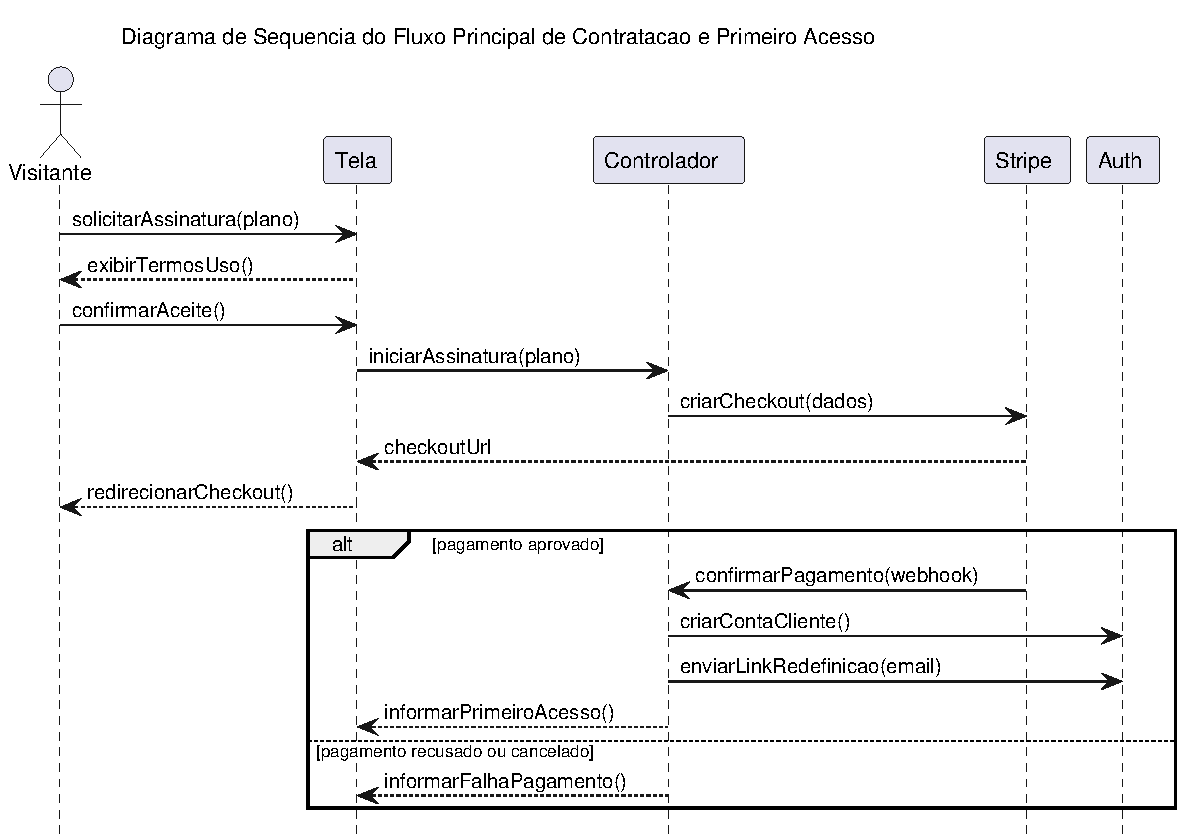
\includegraphics[width=\textwidth]{sequencia_assinatura_primeiro_acesso}
\caption{Diagrama de sequ\^encia do fluxo principal de contrata\c{c}\~ao e primeiro acesso}
\end{figure}

\section{Diagrama de classes}
\begin{figure}[H]
\centering
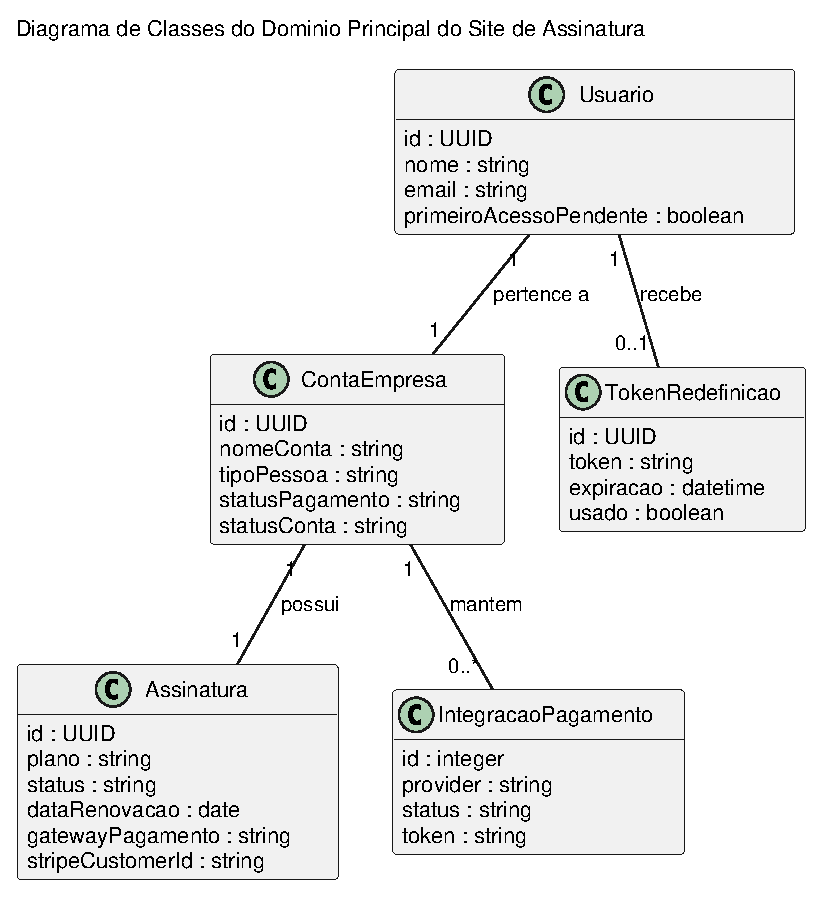
\includegraphics[width=\textwidth]{classes_dominio_assinatura}
\caption{Diagrama de classes do dom\'inio principal do site de assinatura}
\end{figure}
As multiplicidades indicam que cada usu\'ario pertence a uma conta, cada conta possui uma assinatura principal, uma conta pode manter nenhuma ou v\'arias integra\c{c}\~oes e um usu\'ario pode receber um token de redefini\c{c}\~ao quando necess\'ario. O desenho foi mantido no n\'ivel de dom\'inio, com foco nas entidades e nos relacionamentos, em linha com o modelo apresentado pelo professor.

\section{Modelo conceitual simplificado}
\begin{longtable}{>{\raggedright\arraybackslash}p{3.2cm} >{\raggedright\arraybackslash}p{10.3cm}}
\toprule
\textbf{Entidade} & \textbf{Responsabilidade principal} \\
\midrule
Usu\'ario & Representa a identidade autenticada no Supabase, vinculada a e-mail, credenciais de acesso e estado de primeiro acesso. \\
Conta/Empresa & Armazenar\'a os dados centrais do cliente, incluindo situa\c{c}\~ao de pagamento, dados fiscais e refer\^encias da assinatura. \\
Integra\c{c}\~ao da empresa & Guarda a conex\~ao ativa ou inativa com provedores externos, como Mercado Pago. \\
Evento de integra\c{c}\~ao & Registra eventos e payloads relacionados \`as integra\c{c}\~oes para auditoria e diagn\'ostico. \\
Assinatura & Conceito de neg\'ocio representado pelos identificadores do cliente e da assinatura no meio de pagamento. \\
Token de redefini\c{c}\~ao & Elemento utilizado para permitir a cria\c{c}\~ao segura da senha inicial enviada por e-mail ao cliente. \\
Mensagem de suporte & Solicita\c{c}\~ao enviada pelo formul\'ario do site para atendimento ao cliente. \\
\bottomrule
\end{longtable}

\section{Relacionamentos essenciais}
\begin{itemize}
  \item um usu\'ario autenticado estar\'a associado a uma empresa cliente;
  \item uma empresa possuir\'a um estado de cobran\c{c}a que influenciar\'a permiss\~ao de acesso;
  \item uma empresa poder\'a possuir integra\c{c}\~oes com provedores externos;
  \item uma integra\c{c}\~ao poder\'a gerar diversos eventos registrados;
  \item uma empresa poder\'a ser vinculada a um cliente e a uma assinatura.
\end{itemize}

\section{Fluxo principal resumido}
\begin{enumerate}
  \item o visitante acessa a landing page e inicia a contrata\c{c}\~ao;
  \item o site apresentar\'a os termos de uso e somente prosseguir\'a ap\'os o aceite;
  \item o visitante ser\'a redirecionado ao Stripe para preencher os dados iniciais e realizar o pagamento;
  \item com o pagamento aprovado, o backend criar\'a automaticamente a conta do cliente;
  \item o sistema enviar\'a um e-mail para defini\c{c}\~ao ou redefini\c{c}\~ao da senha inicial;
  \item ap\'os definir a senha, o cliente poder\'a acessar a conta e utilizar a plataforma autenticado;
  \item o usu\'ario poder\'a complementar dados fiscais e configurar integra\c{c}\~oes, quando necess\'ario.
\end{enumerate}

\chapter{Descri\c{c}\~ao da arquitetura do sistema e ferramentas utilizadas}

\section{Modelo arquitetural}
O \ProjetoNome{} adotar\'a uma arquitetura web em camadas com abordagem serverless. A \textbf{camada de apresenta\c{c}\~ao} ser\'a composta pelas p\'aginas HTML, folhas de estilo CSS e scripts JavaScript executados no navegador. A \textbf{camada de dom\'inio/aplica\c{c}\~ao} concentrar\'a as regras de neg\'ocio do site de assinatura, como valida\c{c}\~ao do fluxo de contrata\c{c}\~ao, autentica\c{c}\~ao, gest\~ao de conta, controle do status da assinatura e integra\c{c}\~oes. A \textbf{camada de persist\^encia} ser\'a respons\'avel pelo armazenamento dos dados em PostgreSQL por meio do Supabase. Por fim, haver\'a a comunica\c{c}\~ao com \textbf{servi\c{c}os externos}, como Stripe, Mercado Pago e Resend.

Esse modelo foi escolhido por ser adequado a um produto SaaS de pequeno e m\'edio porte, permitindo evolu\c{c}\~ao incremental, baixo acoplamento entre interface e backend e integra\c{c}\~ao simplificada com provedores externos.

\section{Arquitetura l\'ogica}
\begin{figure}[H]
\centering
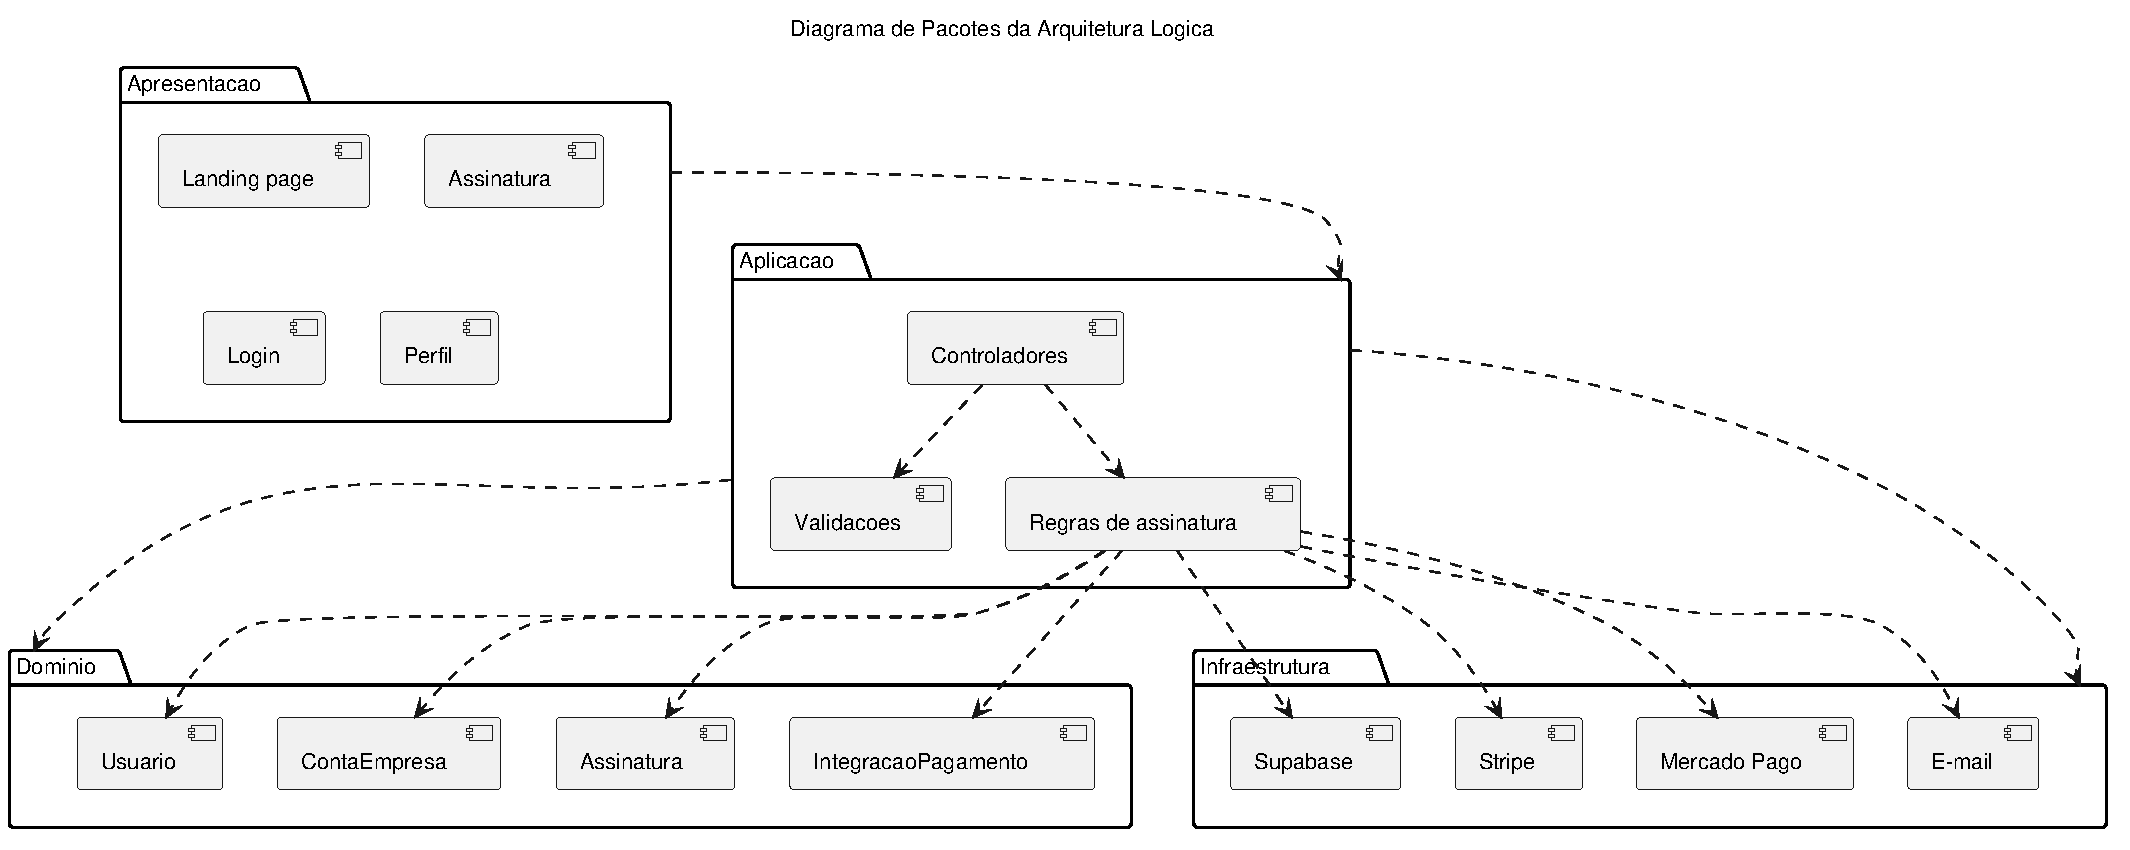
\includegraphics[width=0.92\textwidth]{arquitetura_logica}
\caption{Diagrama de pacotes da arquitetura l\'ogica}
\end{figure}

\section{Arquitetura f\'isica}
\begin{figure}[H]
\centering
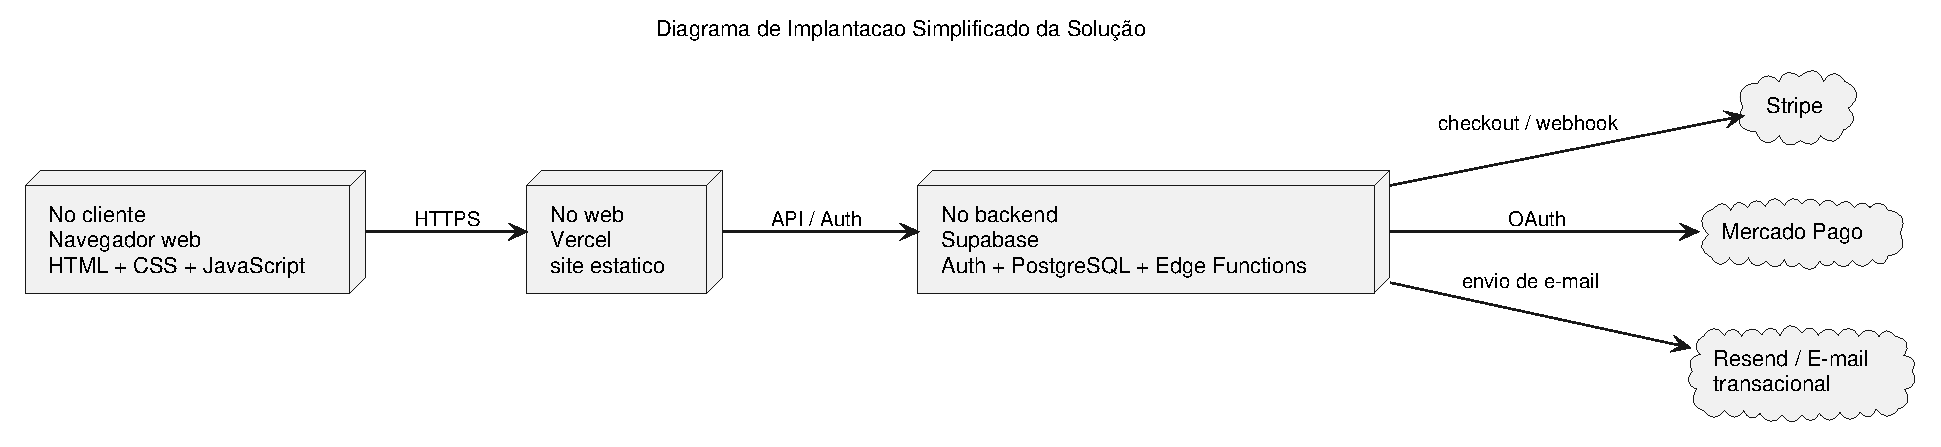
\includegraphics[width=0.92\textwidth]{arquitetura_fisica_implantacao}
\caption{Diagrama de implanta\c{c}\~ao simplificado da solu\c{c}\~ao}
\end{figure}

\section{Ferramentas e tecnologias}
\begin{longtable}{>{\raggedright\arraybackslash}p{3.6cm} >{\raggedright\arraybackslash}p{9.9cm}}
\toprule
\textbf{Tecnologia} & \textbf{Uso no projeto} \\
\midrule
HTML5 & Estrutura das p\'aginas da landing page, assinatura e \'area de conta. \\
CSS3 & Estiliza\c{c}\~ao visual e responsividade da interface. \\
JavaScript & L\'ogica de interface, autentica\c{c}\~ao no cliente e integra\c{c}\~ao com APIs. \\
Supabase & Backend como servi\c{c}o, autentica\c{c}\~ao, banco PostgreSQL e fun\c{c}\~oes serverless. \\
PostgreSQL & Persist\^encia de dados estruturados da aplica\c{c}\~ao. \\
Deno & Execu\c{c}\~ao das Edge Functions do Supabase. \\
Stripe & Pagamento online, assinaturas recorrentes e portal de cobran\c{c}a, previstos para o site de assinatura. \\
Mercado Pago & Integra\c{c}\~ao de pagamento conectada por OAuth. \\
Resend & Envio de e-mails do formul\'ario de suporte. \\
Vercel & Hospedagem do site, conforme o contexto do projeto. \\
Git/GitHub & Versionamento do c\'odigo-fonte e evolu\c{c}\~ao colaborativa. \\
\bottomrule
\end{longtable}

\section{Justificativa das escolhas}
As tecnologias escolhidas atendem ao objetivo de desenvolver um produto web moderno com baixo custo operacional inicial e boa velocidade de entrega. O front-end em HTML, CSS e JavaScript puro reduz depend\^encias e facilita a publica\c{c}\~ao. O Supabase simplifica autentica\c{c}\~ao, fun\c{c}\~oes serverless e persist\^encia. Stripe e Mercado Pago foram considerados porque atendem ao cen\'ario de assinatura e cobran\c{c}a previsto para as pr\'oximas fases, enquanto o uso de PostgreSQL oferece flexibilidade e consist\^encia para evoluir o dom\'inio do sistema.

\section{Considera\c{c}\~oes finais da arquitetura}
Com base no escopo definido e no backlog previsto, a arquitetura do \ProjetoNome{} \'e compat\'ivel com a evolu\c{c}\~ao do produto para novas funcionalidades ligadas \`a assinatura, conta do cliente e integra\c{c}\~oes. O desenho proposto favorece crescimento incremental, desde que a documenta\c{c}\~ao, os testes e as regras de neg\'ocio sejam refinados a cada nova entrega. Entre as pr\'oximas implementa\c{c}\~oes priorit\'arias est\'a justamente o desenvolvimento completo do site de assinatura, que ainda n\~ao foi conclu\'ido nesta etapa do projeto.

\end{document}
